\documentclass[a4paper, czech]{article}

\title{Úloha č.5: Tranzistor MOSFET - V-A charakteristiky a použití jako spínač}
\author{Karolína Andrea Šebestová}
\date{Datum měření: 11.4.2024}

\usepackage[czech]{babel}
\usepackage{indentfirst}
\usepackage{graphicx}
\usepackage{float}
\usepackage[margin=1.5cm]{geometry}
\usepackage{booktabs}
\usepackage{amsmath}
\usepackage{multirow}
\usepackage{colortbl}
\usepackage{array}

\begin{document}

\maketitle

\section{Teoretický úvod}

V této úloze budou měřeny vlastnosti unipolárního tranzistoru MOSFET s indukovaným kanálem typu N (NMOS), jehož princip činnosti je naznačen na Obr. 1.
Základem tranzistoru je polovodičová destička (substrát) typu P, ve které jsou vytvořeny dvě oblasti s vodivostí typu N.
K nim jsou připojeny elektrody source (S) a drain (D).
Hradlo (G - gate) je od substrátu odděleno izolujícím oxidem křemíku ($SiO_2$).
Připojením kladného napětí $U_{GS}$ na hradlo dojde v substrátu k odpuzování majoritních nosičů náboje (tj. děr) a mezi D a S vzniká vodivý kanál (na Obr. 1 černě), kterým mohou procházet elektrony.
Čím větší bude napětí $U_{GS}$, tím bude kanál širší a tím bude větší proud $I_D$ (viz převodní charakteristika na Obr. 2).
Z výstupních charakteristik na Obr. 2 je zřejmé, že proud $I_D$ se zvětšuje také při zvětšování $U_{DS}$.
Pro $U_{DS} > U_{DS_{sat}}$ však přestane proud $I_D$ narůstat.
Při zvyšování $U_{DS}$ totiž zároveň klesá rozdíl potenciálů mezi G a D a v blízkosti D se kanál zužuje (Obr. 1).
Při nulovém rozdílu dojde na straně kolektoru (D) k uzavření kanálu a k saturaci proudu.

\begin{figure}[H]
    \centering
    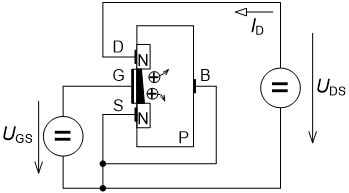
\includegraphics{princip.png}
    \caption{Princip činnosti tranzistoru NMOS s indukovaným kanálem}
\end{figure}

\begin{figure}[H]
    \centering
    
\includegraphics{charakteristiky.png}
    \caption{Charakteristiky tranzistoru NMOS s indukovaným kanálem}
\end{figure}

\pagebreak

\section{Seznam přístrojů}

\begin{enumerate}
    \item Zdroj Agilent E3620A
    \item 2x Multimetr Keysight 34461A
    \item Generátor Agilent 33521A
    \item Osciloskop Agilent DSO-X 2002A
    \item Osciloskopická sonda HP 10074B
\end{enumerate}

\section{Úkoly měření}

\begin{enumerate}
    \item Změřte výstupní charakteristiky tranzistoru BS170, tedy $I_D = f (U_{DS})$ při různých hodnotách $U_{GS} = konst.$ v zapojení podle Obr. 3. Hodnoty napětí $U_{GS}$ volte 0; 2; 2,5; 2,8; 3 V a odečítejte je přímo na displeji laboratorního zdroje E3620A (levý voltmetr tedy nebude použit). Hodnoty $I_D$ a $U_{DS}$ měřte pomocí multimetrů. Napětí $U_{DS}$ nastavujte pomocí regulovatelného zdroje E3620A (druhý kanál) až do hodnoty $U_{CC} = 25 V$. Proměřte jednotlivé charakteristiky v dostatečném počtu bodů pro spojení hladkými křivkami, hodnoty zapište do tabulky a zakreslete do grafu.
    \item Změřte převodní charakteristiku $I_D = f (U_{GS})$ při $U_{DS} = konst.$ opět podle Obr. 3, tedy zapojení ponechte z předchozího úkolu. Nastavte $U_{DS} = 5 V$ (měřte jej multimetrem) a udržujte toto napětí pomocí regulace zdroje $U_{CC}$ během celého měření konstantní. Napětí $U_{GS}$ nastavujte podle displeje zdroje od nuly po maximum, kdy ještě půjde udržet $U_{DS} = 5 V$. Naměřené hodnoty zapište do tabulky a vyneste do grafu. Totéž měření proveďte ještě pro $U_{DS} = 3 V$. 
    \item Zapojte obvod pro spínání tranzistorem NMOS podle Obr. 4. Na generátoru nastavte obdélníkový průběh (Waveforms, Square), kmitočet 2 MHz, mezivrcholovou hodnotu napětí 5 V špička-špička (na generátoru nastavte 2,5 Vpp)  a ofset 2,5 V (na generátoru 1,25 V). Napětí $U_{CC}$ nastavte na 15 V. Signál do druhého kanálu osciloskopu přivádějte pomocí osciloskopické sondy (s přenosem 1:10, nezapomeňte ji nastavit na osciloskopu jako v minulých úlohách). Černé krokodýlky koaxiálních kabelů a sondy připojujte k zemnímu, tedy ve schématu spodnímu, vodiči. Z osciloskopu obkreslete či elektronicky vložte do protokolu vstupní a výstupní průběhy napětí a odečtěte časové posuny mezi vstupem a výstupem, jak je naznačeno v Obr. 5. Tyto posuny vyznačte v průbězích.
\end{enumerate}

\begin{figure}[H]
    \centering
    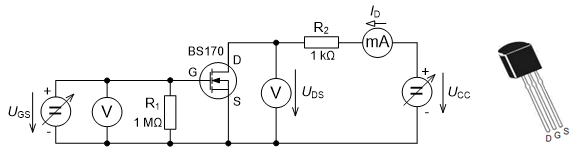
\includegraphics{zapojeni1.png}
    \caption{Zapojení pro měření charakteristik tranzistoru NMOS}
\end{figure}

\begin{figure}[H]
    \centering
    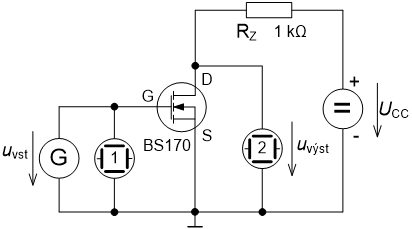
\includegraphics[width=0.4\textwidth]{zapojeni2.png}
    \caption{Zapojení tranzistoru NMOS jako spínač}
\end{figure}

\begin{figure}[H]
    \centering
    
\includegraphics{prubehy.png}
    \caption{Průběhy napětí při spínání tranzistoru NMOS}
\end{figure}

\section{Naměřené hodnoty}

Tato sekce byla rozdělena do několika podsekcí pro jednotlivé měření.
V první podsekci se nachází jedna tabulka obsahující naměřené hodnoty pěti výstupních charakteristik.
Ve druhé podsekci se nachází tabulka s naměřenými hodnotami dvou převodních charakteristik.
V poslední podsekci se nachází časové průběhy vstupního a výstupního napětí tranzistoru zapojeného jako spínač.

Slovní popis symbolů veličin:
$U_{GS}$ - hradlové napětí (gate - source);
$U_{DS}$ - kanálové napětí (drain - source);
$I_D$ - proud tekoucí kanálem;
$t_{df}$ - doba zpoždění sestupné hrany;
$t_{f}$ - délka sestupné hrany;
$t_{dr}$ - doba zpoždění náběžné hrany;
$t_{r}$ - délka náběžné hrany


\subsection{Výstupní charakteristiky tranzistoru NMOS}

\begin{table}[H]
    \centering 
    \begin{tabular}{cccccccccc}
    \toprule
        \multicolumn{2}{c}{$U_{GS} = 0V$} & \multicolumn{2}{c}{$U_{GS} = 2V$} & \multicolumn{2}{c}{$U_{GS} = 2,5V$} & \multicolumn{2}{c}{$U_{GS} = 2,8V$} & \multicolumn{2}{c}{$U_{GS} = 3V$} \\ 
        $U_{DS}\ (V)$ & $I_D\ (\mu A)$ & $U_{DS}\ (V)$ & $I_D\ (\mu A)$ & $U_{DS}\ (V)$ & $I_D\ (mA)$ & $U_{DS}\ (V)$ & $I_D\ (mA)$ & $U_{DS}\ (V)$ & $I_D\ (mA)$ \\
        \midrule
        0  & 0     & 0    & 0      & 0     & 0     & 0    & 0     & 0     & 0     \\
        1  & 0,098 & 0,05 & 37,73  & 0,05  & 1,61  & 0,05 & 4,74  & 0,025 & 3,89  \\
        2  & 0,197 & 0,1  & 49,82  & 0,1   & 2,343 & 0,1  & 8,07  & 0,05  & 7,44  \\
        3  & 0,297 & 0,25 & 58,18  & 0,25  & 3,216 & 0,25 & 13,3  & 0,075 & 10,6  \\
        4  & 0,397 & 0,5  & 61,71  & 0,5   & 3,526 & 0,5  & 15,7  & 0,1   & 13,46 \\
        5  & 0,497 & 1    & 62,87  & 1     & 3,684 & 1    & 16,76 & 0,125 & 16,17 \\
        6  & 0,596 & 2    & 65,27  & 2     & 3,845 & 2    & 17,91 & 0,15  & 18,51 \\
        7  & 0,695 & 3    & 67,2   & 3     & 3,99  & 3    & 18,79 & 0,175 & 20,4  \\
        8  & 0,795 & 4    & 69,08  & 4     & 4,11  & 3,5  & 19,66 & 0,2   & 22,17 \\
        9  & 0,894 & 5    & 71,03  & 5     & 4,23  & 3,77 & 20,88 & 0,21  & 22,85 \\
        10 & 0,994 & 6    & 72,99  & 6     & 4,4   &      &       & 0,22  & 23,46 \\
        11 & 1,093 & 7    & 75,11  & 7     & 4,55  &      &       & 0,23  & 24,13 \\
        12 & 1,192 & 8    & 77,35  & 8     & 4,71  &      &       & 0,238 & 24,51 \\
        13 & 1,292 & 9    & 79,71  & 9     & 4,91  &      &       &       &       \\
        14 & 1,392 & 10   & 82,29  & 10    & 5,1   &      &       &       &       \\
        15 & 1,493 & 11   & 84,97  & 11    & 5,31  &      &       &       &       \\
        16 & 1,592 & 12   & 87,79  & 12    & 5,53  &      &       &       &       \\
        17 & 1,691 & 13   & 90,78  & 13    & 5,86  &      &       &       &       \\
        18 & 1,791 & 14   & 93,92  & 14    & 6,14  &      &       &       &       \\
        19 & 1,89  & 15   & 97,44  & 15    & 6,43  &      &       &       &       \\
        20 & 1,989 & 16   & 101,25 & 16    & 6,76  &      &       &       &       \\
        21 & 2,09  & 17   & 105,22 & 17    & 7,17  &      &       &       &       \\
        22 & 2,188 & 18   & 109,38 & 17,38 & 7,5   &      &       &       &       \\
        23 & 2,287 & 19   & 113,96 &       &       &      &       &       &       \\
        24 & 2,387 & 20   & 118,66 &       &       &      &       &       &       \\
        25 & 2,486 & 21   & 123,91 &       &       &      &       &       &       \\
           &       & 22   & 129,51 &       &       &      &       &       &       \\
           &       & 23   & 135,42 &       &       &      &       &       &       \\
           &       & 24   & 141,73 &       &       &      &       &       &       \\
           &       & 25   & 148,74 &       &       &      &       &       &       \\
    \bottomrule
    \end{tabular}
    \caption{Naměřené hodnoty výstupních charakteristik tranzistoru BS170 při několika hodnotách $U_{GS}$}
\end{table}

\subsection{Převodní charakteristiky tranzistoru NMOS}

\begin{table}[H]
    \centering
    \begin{tabular}{ccc}
        \toprule
        \multirow{2}{*}{$U_{GS}\ (V)$}& $U_{DS}=5V$ & $U_{DS}=3V$ \\
         & $I_D\ (mA)$ & $I_D\ (mA)$ \\
        \midrule
        0   & 0,00  & 0,00  \\
        1   & 0,00  & 0,00  \\
        2   & 0,08  & 0,07  \\
        2,1 & 0,21  & 0,18  \\
        2,2 & 0,48  & 0,47  \\
        2,3 & 1,09  & 1,00  \\
        2,4 & 2,21  & 2,10  \\
        2,5 & 4,30  & 3,93  \\
        2,6 & 7,63  & 7,03  \\
        2,7 & 12,73 & 11,82 \\
        2,8 & 20,12 & 18,49 \\
        \bottomrule
    \end{tabular}
    \caption{Naměřené hodnoty převodních charakteristik tranzistoru BS170 při dvou hodnotách $U_{DS}$}
\end{table}

\pagebreak

\subsection{Časové posuny při zapojení tranzistoru NMOS jako spínač}

Na následujících čtyřech průbězích jsou zobrazeny časové průběhy z osciloskopu, kde jsou vyznačeny jednotlivé časové posuny.
Body, mezi kterými bylo měření provedeno jsou znázorněny červenými šipkami.
Konkrétní naměřená časová hodnota je zvýrazněna červeným rámečkem.
Všechny naměřené časové hodnoty jsou na konci podsekce uvedeny ve společné tabulce. 

\begin{figure}[H]
    \centering
    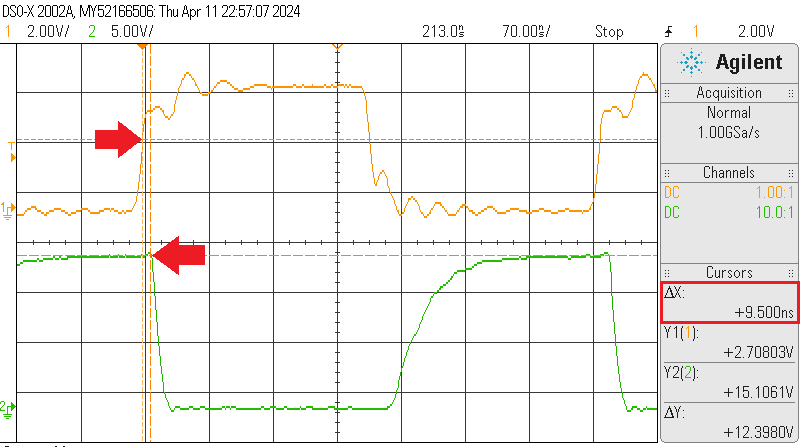
\includegraphics[width=0.7\textwidth]{t_df.png}
    \caption{Vstupní a výstupní průběhy napětí z osciloskopu - vyznačen časový posun $t_{df}$}
\end{figure}

\begin{figure}[H]
    \centering
    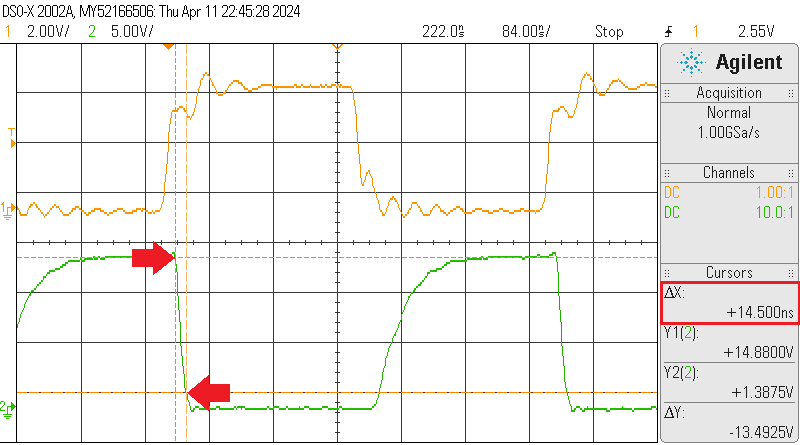
\includegraphics[width=0.7\textwidth]{t_f.png}
    \caption{Vstupní a výstupní průběhy napětí z osciloskopu - vyznačen časový posun $t_{f}$}
\end{figure}

\begin{figure}[H]
    \centering
    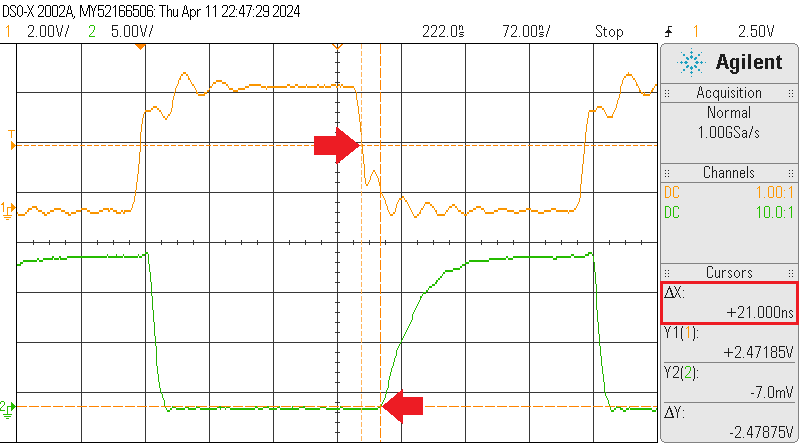
\includegraphics[width=0.7\textwidth]{t_dr.png}
    \caption{Vstupní a výstupní průběhy napětí z osciloskopu - vyznačen časový posun $t_{dr}$}
\end{figure}

\begin{figure}[H]
    \centering
    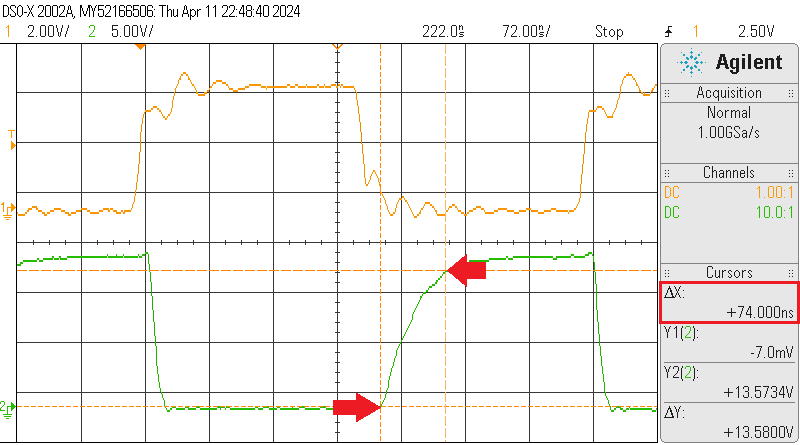
\includegraphics[width=0.7\textwidth]{t_r.png}
    \caption{Vstupní a výstupní průběhy napětí z osciloskopu - vyznačen časový posun $t_{r}$}
\end{figure}

\begin{table}[H]
    \centering
    \begin{tabular}{cccc}
        \toprule
        $t_{df}\ (ns)$ & $t_{f}\ (ns)$ & $t_{dr}\ (ns)$ & $t_{dr}\ (ns)$ \\
        \midrule
        9,5 & 14,5 & 21 & 74 \\
        \bottomrule
    \end{tabular}
    \caption{Naměřené hodnoty časových posunů tranzistoru BS170 zapojeného jako spínač}
\end{table}

\pagebreak

\section{Grafy}

Jednotlivé výstupní charakteristiky byly vyneseny do společného grafu jako závislost proudu tekoucího kanálem $I_D$ na kanálovém napětí $U_{DS}$.

\begin{figure}[H]
    \centering
    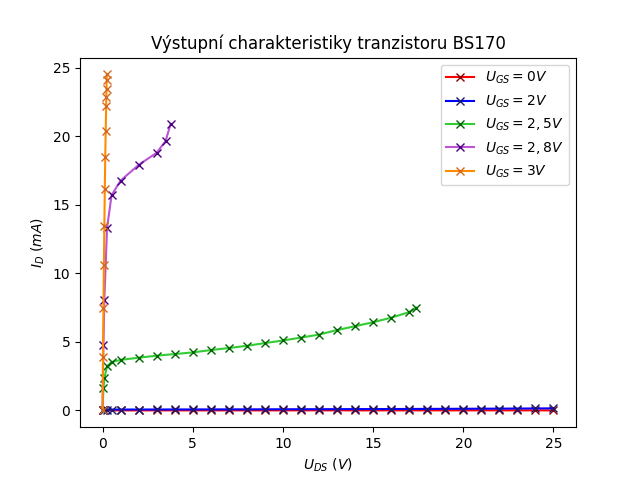
\includegraphics[width=\textwidth]{vystupni.png}
    \caption{Naměřené výstupní charakteristiky tranzisotru BS170 vyneseny do společného grafu}
\end{figure}

\pagebreak

Naměřené převodní charakteristiky byly vyneseny do společného grafu jako závislost proudu protékajícího kanálem $I_D$ na hradlovém napětí $U_{GS}$.

\begin{figure}[H]
    \centering
    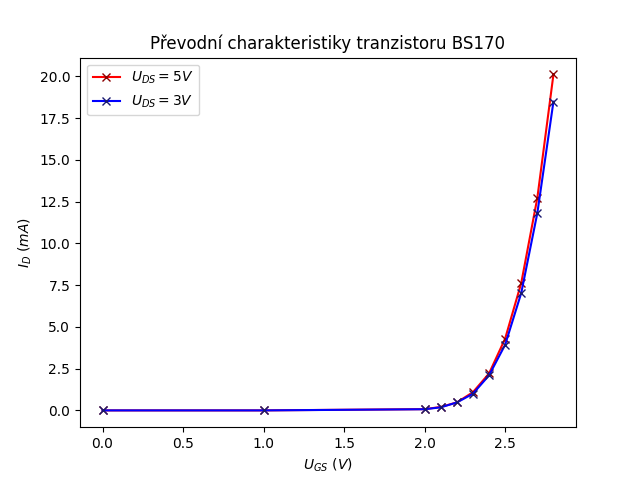
\includegraphics{prevodni.png}
    \caption{Naměřené převodní charakteristiky tranzisotru BS170 vyneseny do společného grafu}
\end{figure}

\section{Závěr}

Jako první jsme měřili výstupní charkateristiky tranzistoru BS170 při různých hodnotách $U_{GS} = konst.$
Napětí $U_{DS}$ jsme pro jednotlivé charakteriky nastavovali na různé hodnoty jen dokud $U_{CC} = 25V$.
Naměřené hodnoty všech charakteristik byly poté vyneseny do společného grafu.
Výsledek měření však odpovídal očekáváním jen částečně.
První charakteristika při $U_{GS} = 0V$ má lineární charakter, to však v grafu při zvoleném měřítku není vidět.
Druhá charakteristika při $U_{GS} = 2V$ má očekávaný tvar, ale opět se v grafu jeví jako horizontální přímka kvůli zvolenému měŕítku.
Následující charakteristiky jsou "ořezané"\ zprava.
To proto, že jsme počas měření dosáhli na maximální zadané napětí $U_{CC} = 25V$ poměrně brzy.
V poslední měřené charaktersitice z tohoto důvodu není vidět ani její ohyb.
V charakteristikách při $U_{GS} = 2,5V$, $2,8V$ a $3V$ je také patrný exponenciální růst proudu $I_D$ tam, kde by jsme očekávali pouze nepatrný růst.
Tento jev je způsoben teplotní závislostí elektronických součástek použitých pro měření.
Během měření jsme také pozorovali velké zahřívání použitých součástek při dotyku rukou.

Ve druhém měření jsme měřili převodní charakteristiky tranzisoru BS170 při $U_{DS} = konst.$
Měření jsme prováděli jen do maximální hodnoty $U_{GS}$, kdy ještě šlo udržet zadané konstantní napětí $U_{DS}$.
Naměřené hodnoty byly opět vyneseny do společného grafu.
Naměřené charakteristiky jeví tvar exponenciálního charakteru, i když naše očekávání bylo více lineární.
Tato neshoda je opět způsobena teplotními závislostmi zvolených součástek a opět jsme během měření pozorovali velké zahřívání součástek při dotyku prstem.

V posledním měření jsme se věnovali obvodu s tranzistorem BS170 zapojeným jako spínač.
Podstatou tohoto měření bylo prozkoumat jednotlivé časové posuny mezi vstupním a výstupním napěťovým průběhem obvodu a taktéž doby trvání jednotlivých hran výstupního průběhu.
Významným pozorovaným jevem bylo, že náběžná i sestupní hrana výstupního průběhu byla za vstupním průběhem opožděna o několik nanosekund.
Dále jsme měřili délky jednotlivých hran výstupního signálu. Přičemž bylo patrné, že sestupná hrana trvá relativně krátce, avšak náběžná hrana má délku několik desítek nanosekund a její tvar připomíná nabíjení kondenzátoru.


\end{document}